%# -*- coding:utf-8 -*-
\section{研究背景}

\begin{frame}
\frametitle{冠心病病理}
\begin{itemize}
  \item 冠心病病理: 
  \begin{enumerate}[A]
    \item 由于冠状动脉中的血流受阻,导致自受阻位置以下心肌长期缺氧,最终使其坏死
    \item 受阻的冠状动脉内部情况,斑块固着于血管内壁,致使血管横截面积明显缩小,血流受阻
  \end{enumerate}
\end{itemize}
\begin{figure}[t]
\centering
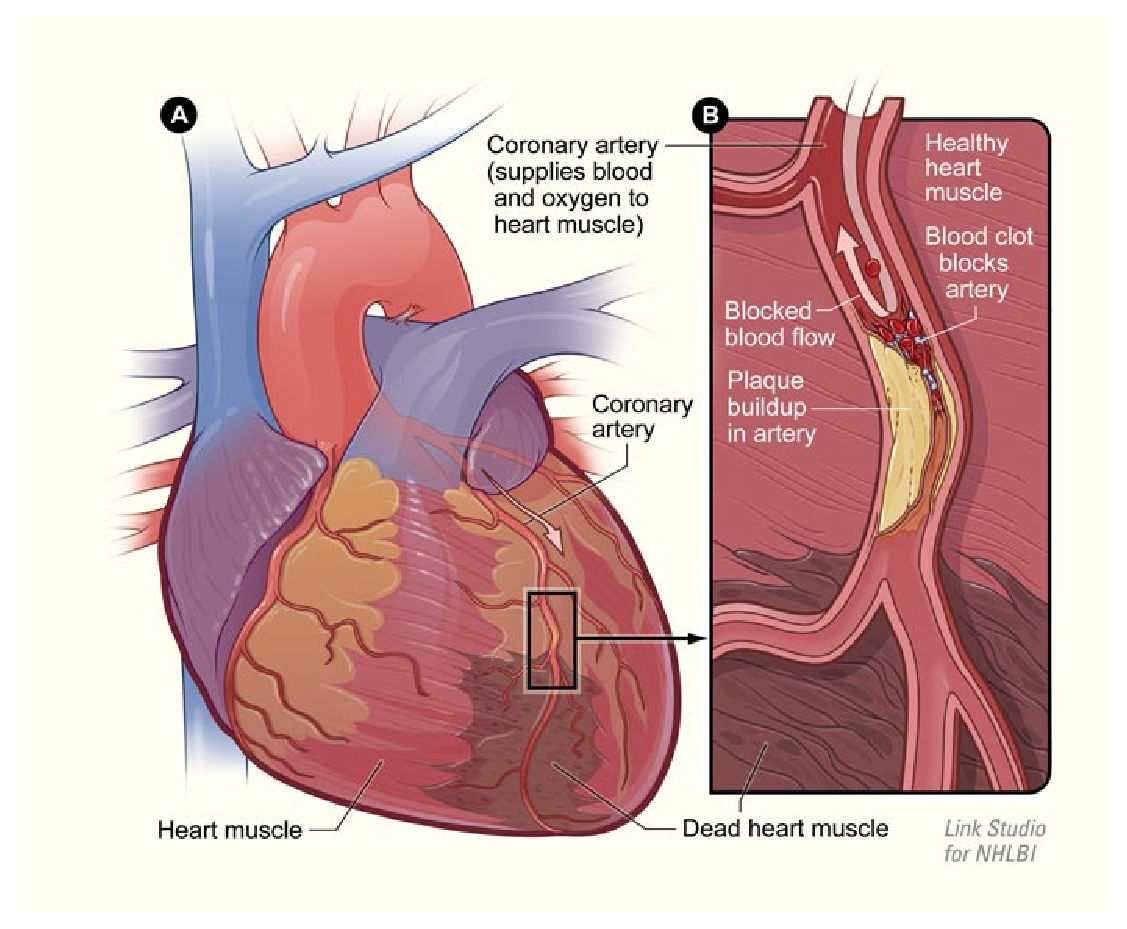
\includegraphics[height=130pt]{../../Figures/background/heart_attack_large.eps}
\caption[冠心病病理]{图片来自:\url{http://www.nhlbi.nih.gov/index.html}}
% \label{fig:heart_attack}
\end{figure}
\end{frame}

\begin{frame}
\frametitle{冠状动脉介入术}
\begin{columns}[onlytextwidth]
\begin{column}{0.4\textwidth}
\begin{figure}[t]
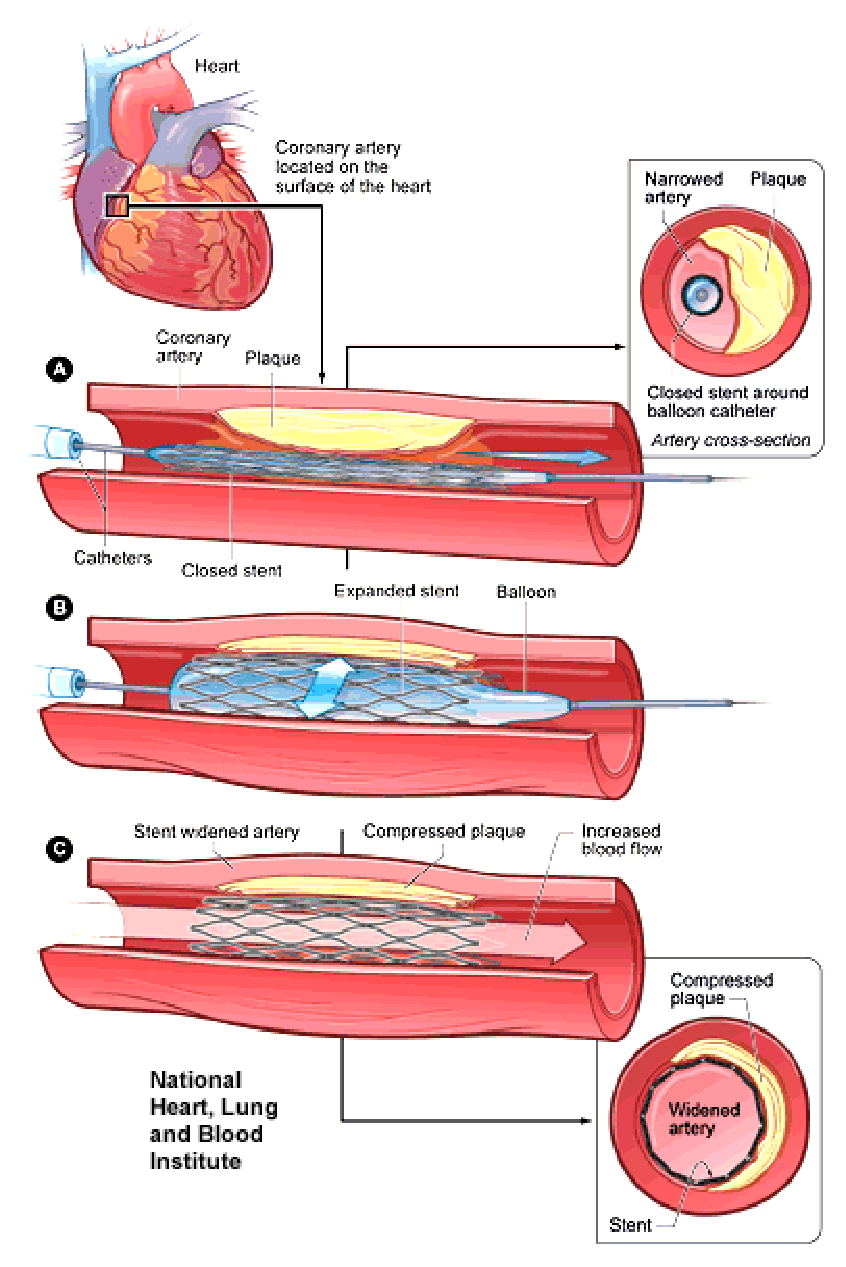
\includegraphics[height=170pt]{../../Figures/background/phauthuatmachmau_stent.eps}
\caption[冠状动脉介入术]{图片来自:\\\url{http://www.nhlbi.nih.gov/index.html}}
\end{figure}
\end{column}
\begin{column}{0.5\textwidth}
\begin{itemize}
\item \textbf{冠状动脉介入术}: 
\begin{itemize}
\item \footnotesize{重建冠状动脉血运的微创介入手术}
\end{itemize}
\item \textbf{主要步骤}:
\begin{enumerate}[A]
\item \footnotesize{将载有气囊的导管沿主动脉送至病灶位置}
\item \footnotesize{向气囊注入空气使其膨胀,迫使气囊外的支架扩张}
\item \footnotesize{通过导管抽出气囊内的空气使其收缩后撤出}
\end{enumerate}
\end{itemize}
\begin{itemize}
\item \textbf{相较于传统手术的优势}
\begin{itemize}
% \setlength{\itemindent}{-.1in}
\item 创口微小
\item 痛苦减轻
\item 较短的手术时间
\item 并发症发生率低
\item 术后恢复快
\end{itemize}
\end{itemize}
\end{column}
\end{columns}
\end{frame}

\begin{frame}
\begin{itemize}
  \item “师傅-学徒”模式的技艺传承: 
  \begin{enumerate}[A]
    \item 手工艺的传承
    \item 医学技术的传承
  \end{enumerate}
\end{itemize}
\begin{figure}
\begin{minipage}[t]{0.8\linewidth}
\centering
% top
\subfigure[]{

\includegraphics[height=60pt]{../../Figures/background/220px-Apprenticeship.eps}
\quad

\includegraphics[height=60pt]{../../Figures/background/220px-Medieval_baker.eps}
}
% bottom
\subfigure[]{
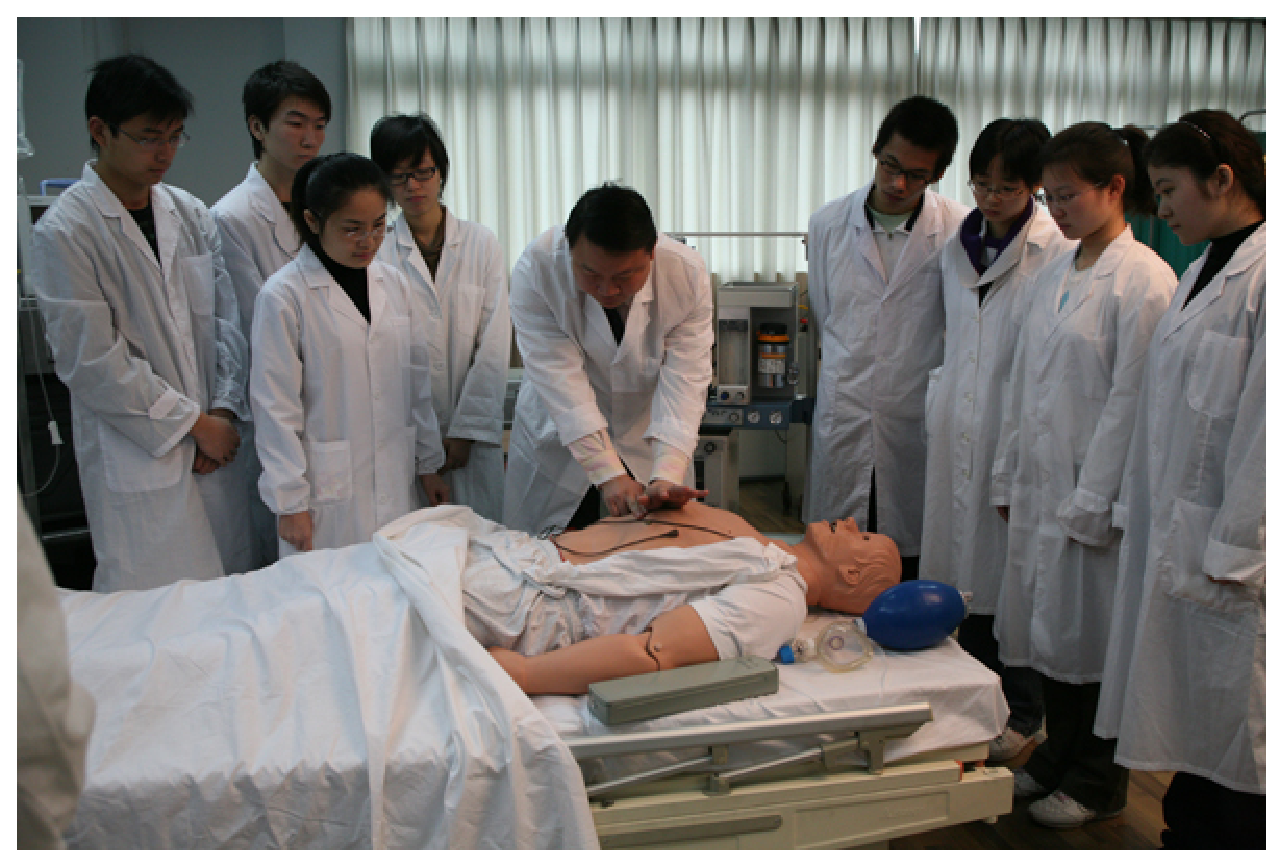
\includegraphics[height=70pt]{../../Figures/background/clinical_training_center.eps}
\quad
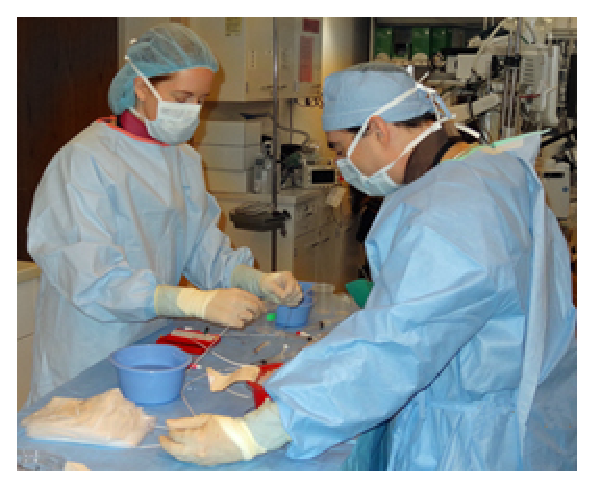
\includegraphics[height=70pt]{../../Figures/background/cath_lab.eps}
}	
\end{minipage}
\end{figure}
\end{frame}

\begin{frame}
\begin{itemize}
  \item 微创血管介入手术机器人系统: 
  \begin{enumerate}
    \item 机器人系统外观
    \item 机器人控制系统
  \end{enumerate}
\end{itemize}
\begin{columns}[b,onlytextwidth]
\begin{column}{.5\textwidth}
\begin{figure}[t]
\centering
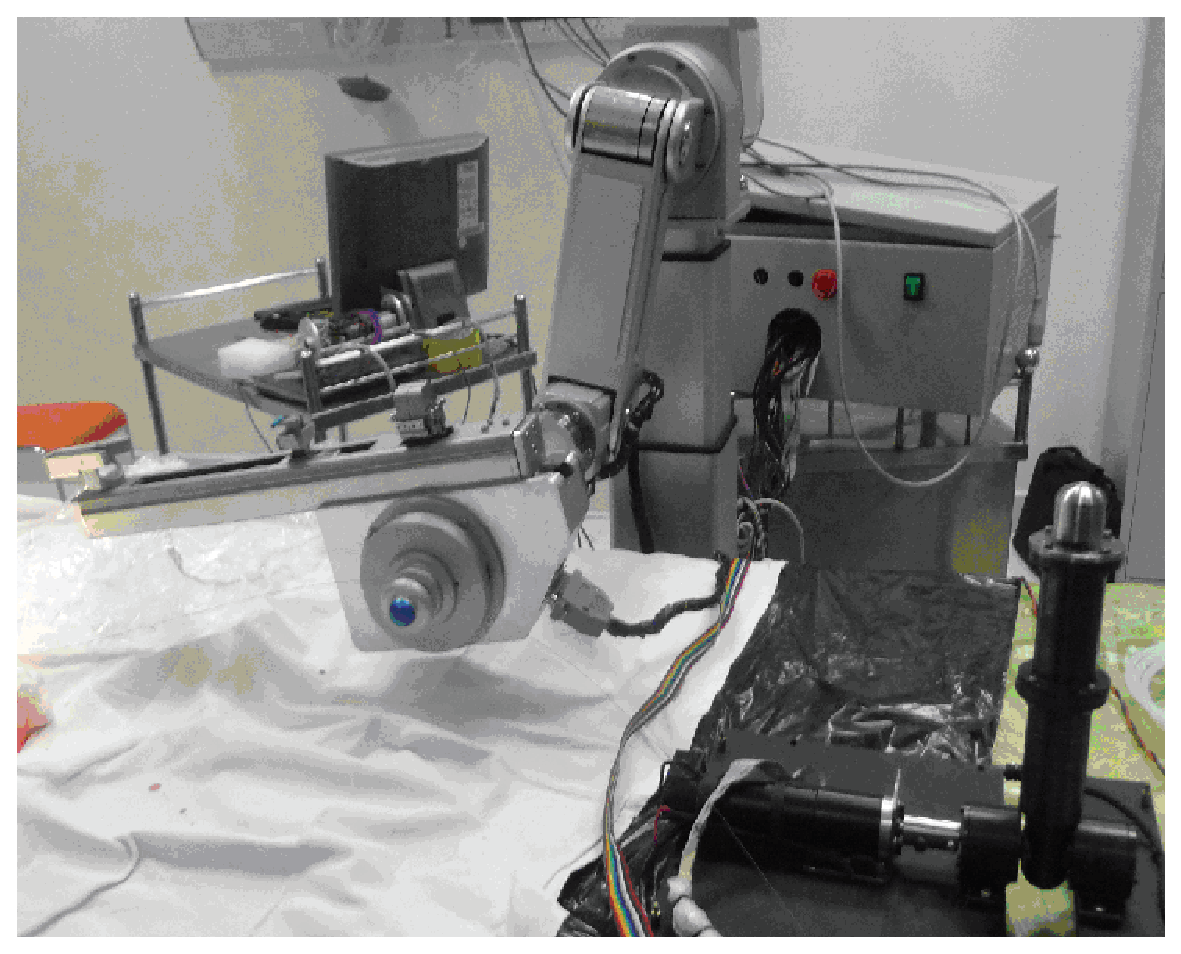
\includegraphics[height=100pt]{../../Figures/background/robot.eps}
\end{figure}
\end{column}
\begin{column}{.5\textwidth}
\begin{figure}[t]
\centering
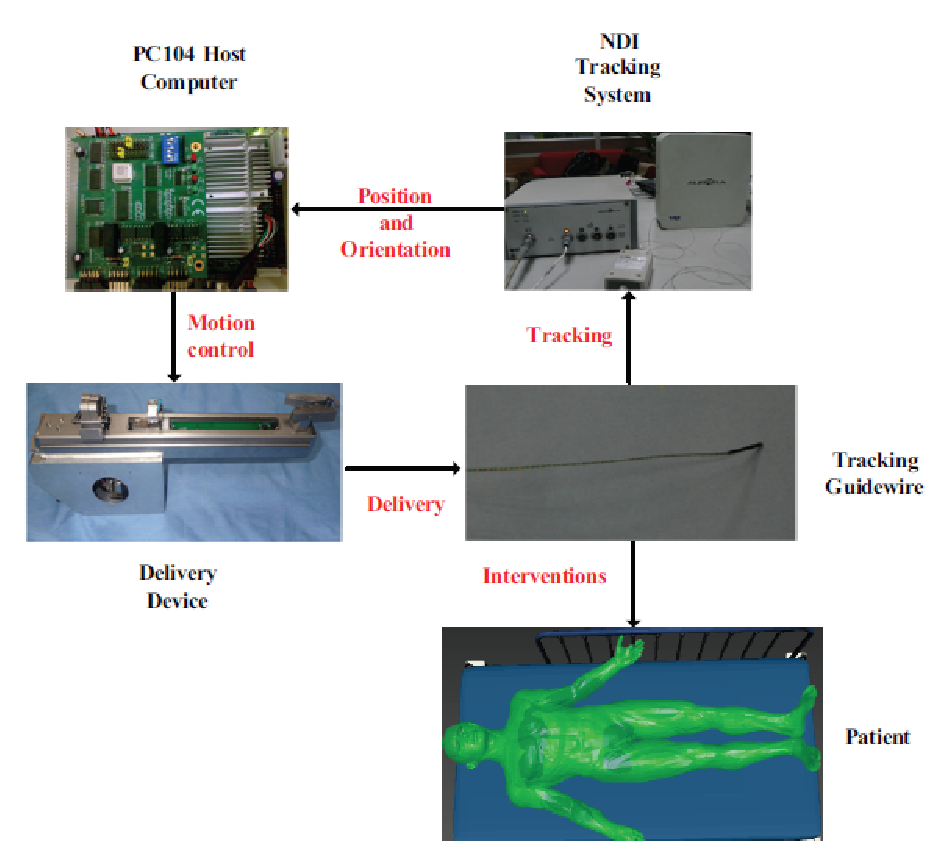
\includegraphics[height=100pt]{../../Figures/background/robot_arch.eps}
\end{figure}
\end{column}
\end{columns}
\end{frame}

\begin{frame}
\begin{itemize}
  \item 微创血管介入手术仿真系统: 
  % \begin{enumerate}
    % \item 机器人外观
    % \item 机器人控制系统
  % \end{enumerate}
\end{itemize}
% \begin{columns}[b,onlytextwidth]
% \begin{column}{.5\textwidth}
\begin{figure}[t]
\centering
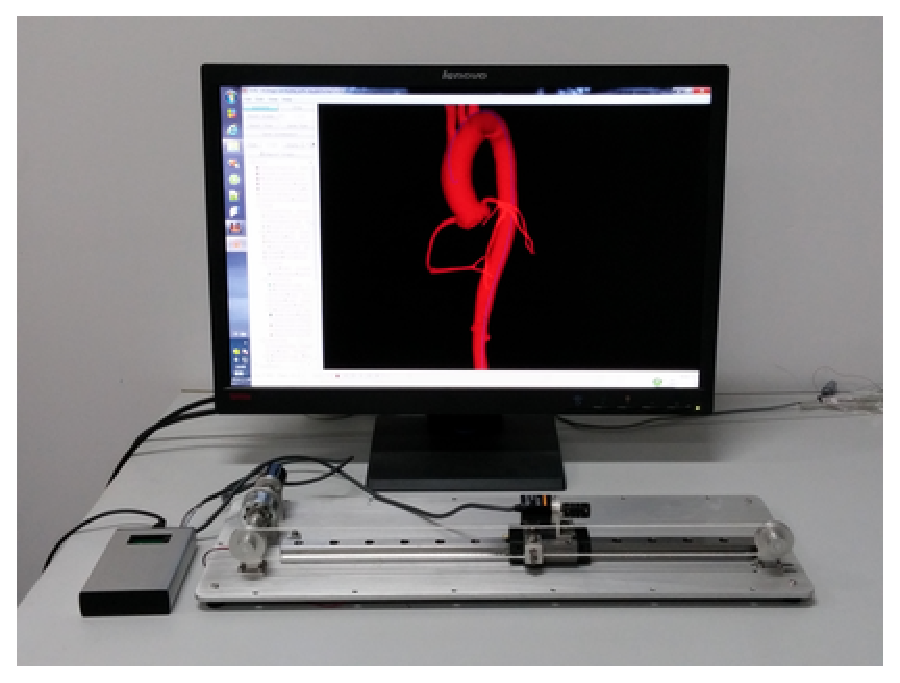
\includegraphics[height=130pt]{../../Figures/background/simulator.eps}
\end{figure}
% \end{column}
% \begin{column}{.5\textwidth}
% \begin{figure}[t]
% \centering
% \input{../../FigureSrc/background/architecture_utf8}
% \end{figure}
% \end{column}
% \end{columns}
\end{frame}

\begin{frame}
\begin{itemize}
  \item 微创血管介入手术机器人系统的主要功能: 
  \begin{enumerate}
    \item 虚拟解剖环境
    \item 虚拟手术工具
    \item 触觉接口
  \end{enumerate}
\end{itemize}
\begin{columns}[b,onlytextwidth]
\begin{column}{.25\textwidth}
\begin{figure}[t]
\centering
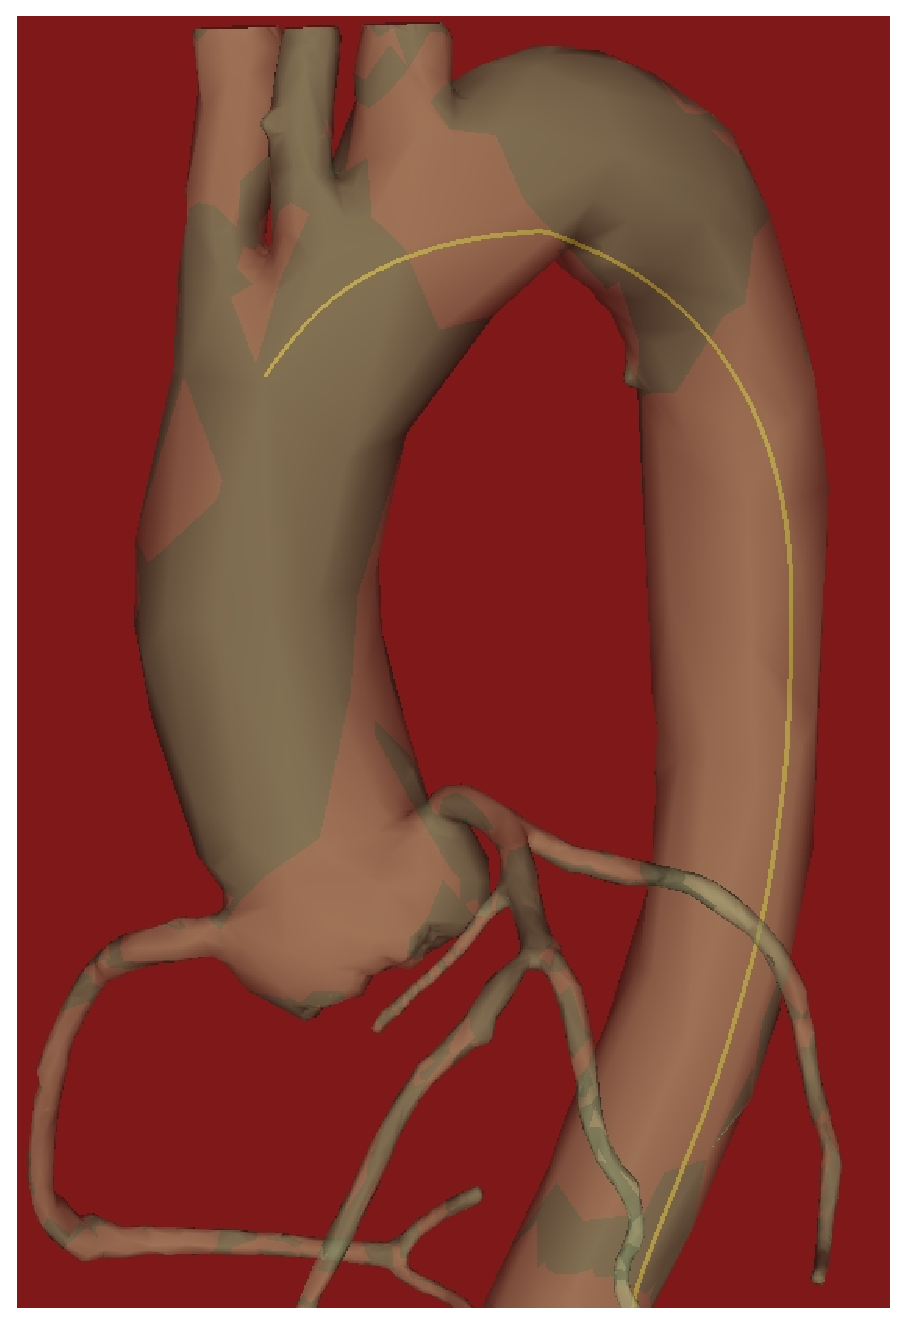
\includegraphics[height=1.0in]{../../Figures/background/simulation2.eps}
% 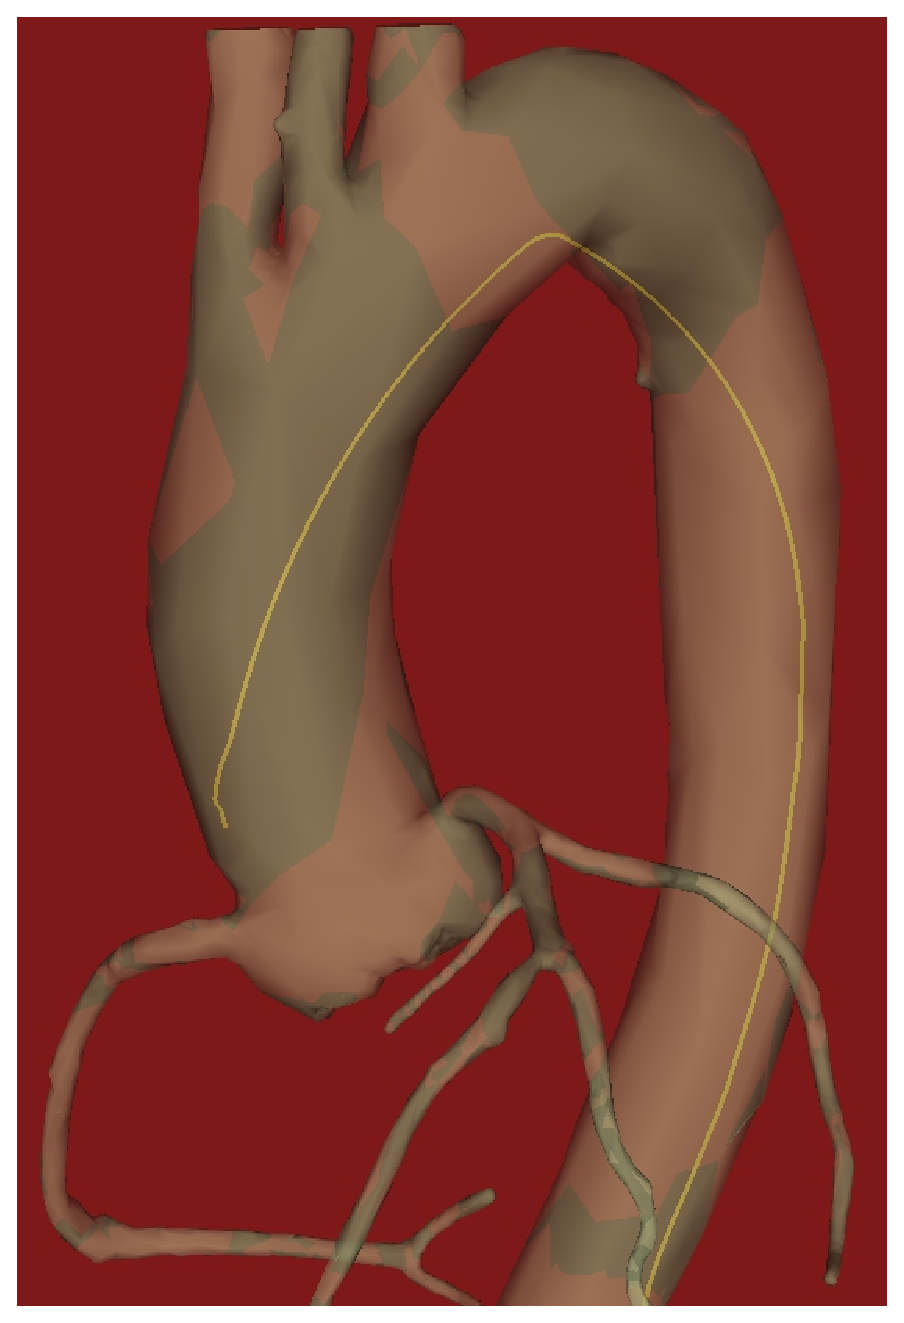
\includegraphics[height=1.0in]{../../Figures/background/simulation.eps}
% 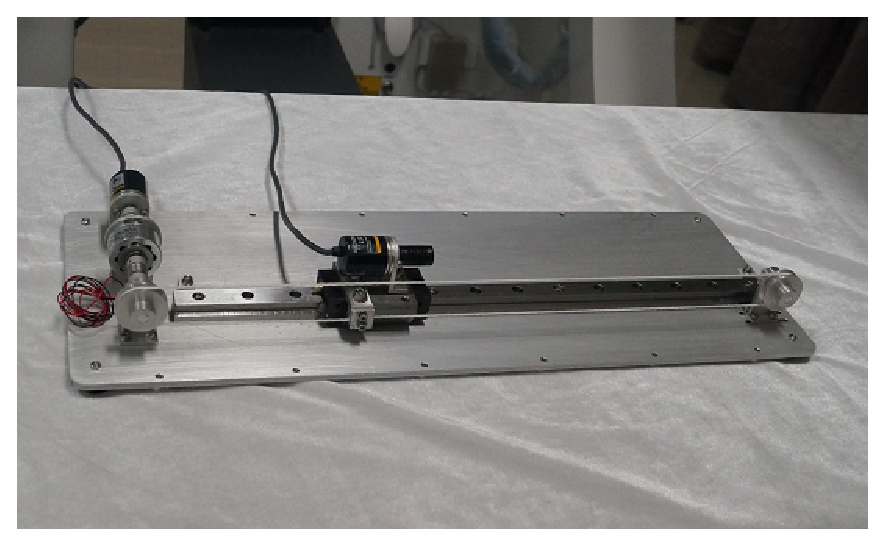
\includegraphics[height=1.0in]{../../Figures/background/interface.eps}
\end{figure}
\end{column}
\begin{column}{.25\textwidth}
\begin{figure}[t]
\centering
% 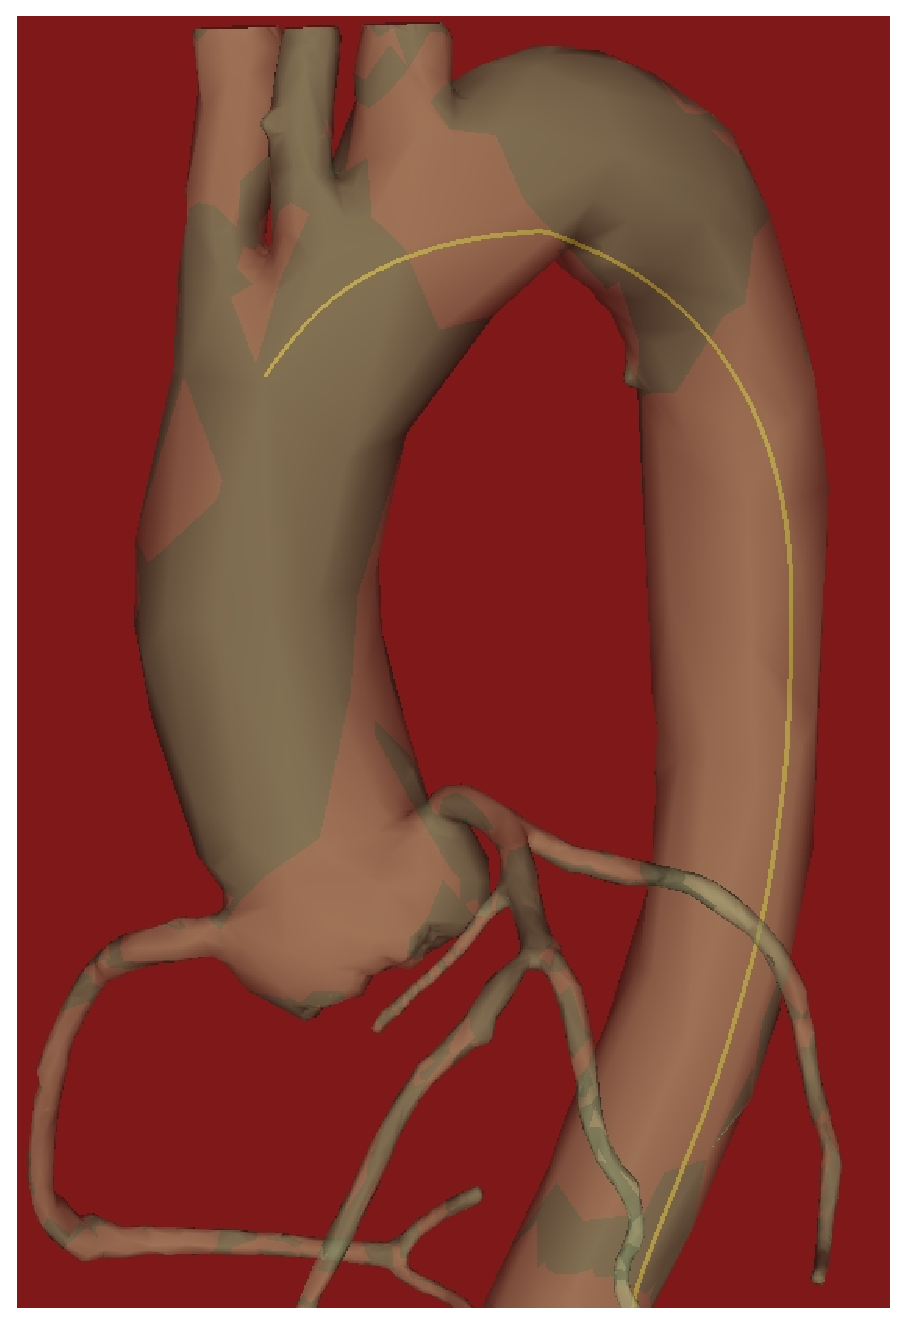
\includegraphics[height=1.0in]{../../Figures/background/simulation2.eps}
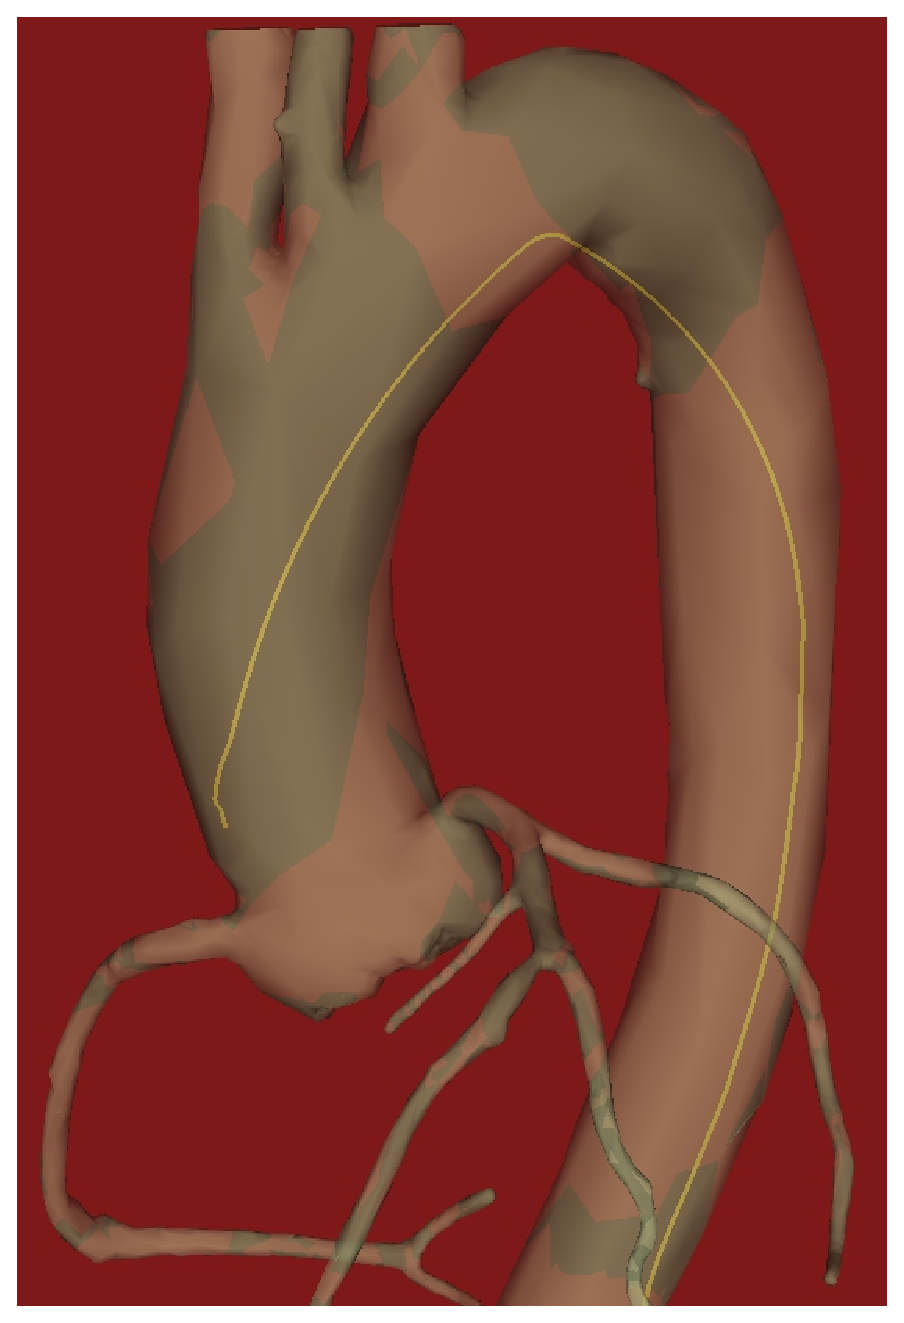
\includegraphics[height=1.0in]{../../Figures/background/simulation.eps}
% 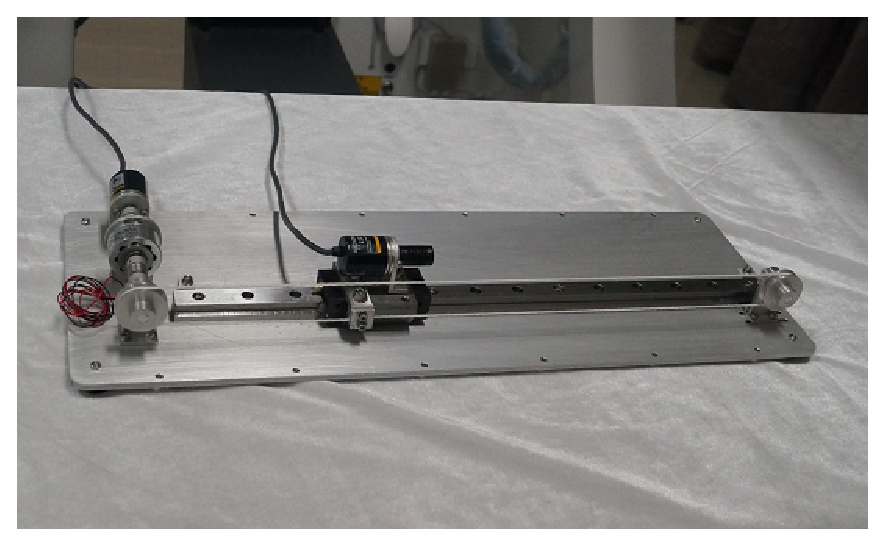
\includegraphics[height=1.0in]{../../Figures/background/interface.eps}
\end{figure}
\end{column}
\begin{column}{.5\textwidth}
\begin{figure}[t]
\centering
% 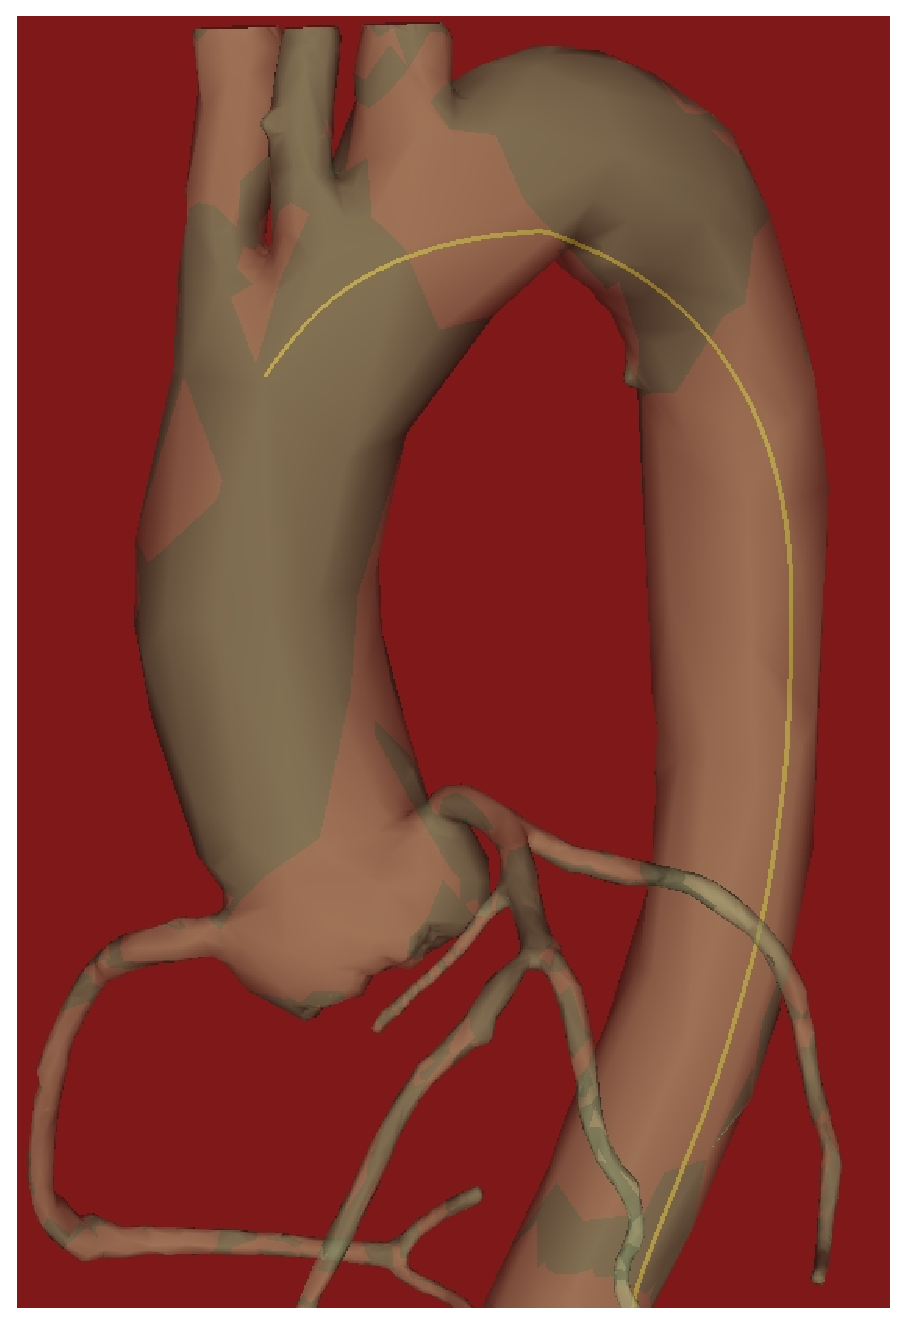
\includegraphics[height=1.0in]{../../Figures/background/simulation2.eps}
% 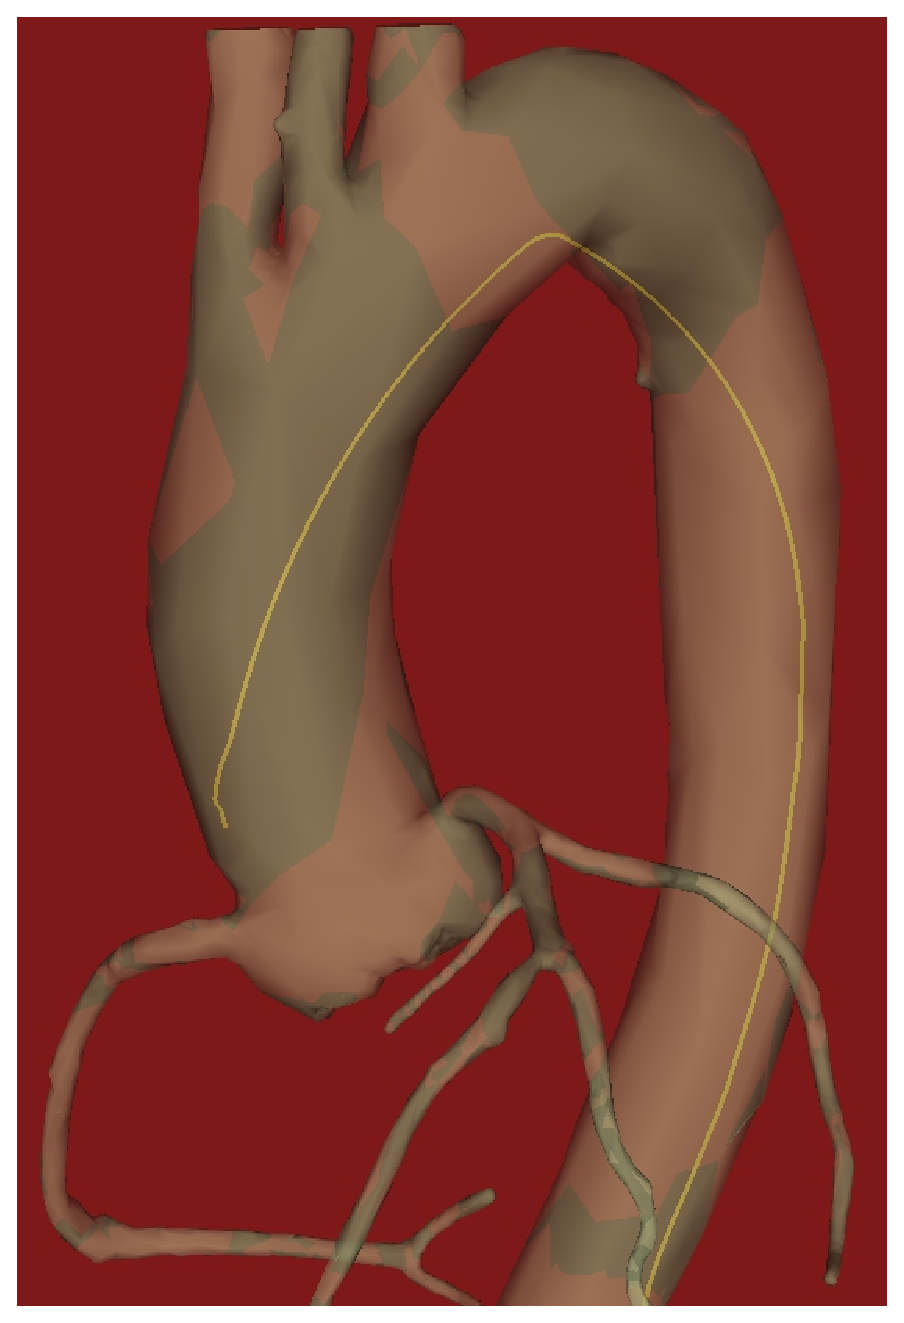
\includegraphics[height=1.0in]{../../Figures/background/simulation.eps}
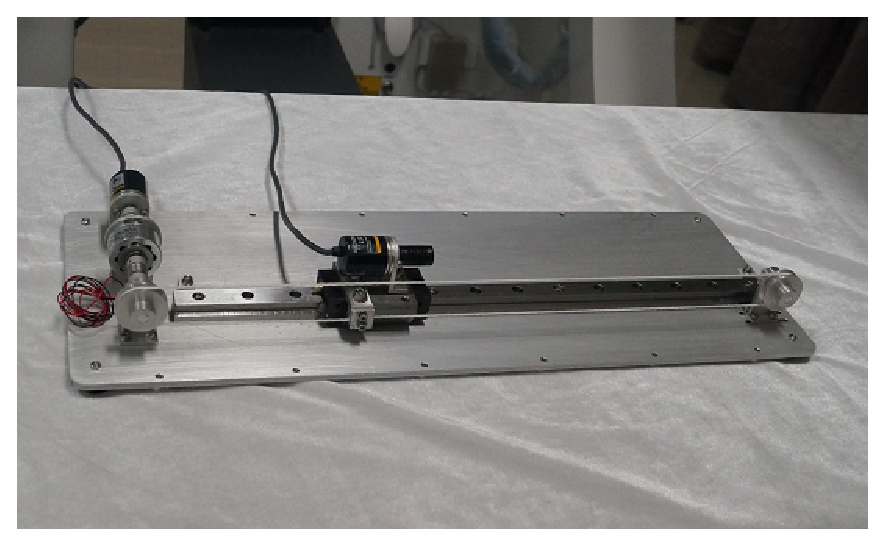
\includegraphics[height=1.0in]{../../Figures/background/interface.eps}
\end{figure}
\end{column}
\end{columns}
\end{frame}